\documentclass[a4paper,10pt,titlepage]{article}

\usepackage{geometry}
\usepackage{amsmath}
\usepackage{amssymb}
\usepackage{txfonts}
\usepackage{microtype}
\usepackage{epsfig}
\usepackage{graphicx}
\usepackage{moreverb}
\usepackage{hyperref}
\usepackage{listings}
\usepackage{xcolor}
\usepackage{textcomp}
\definecolor{listinggray}{gray}{0.98}
\definecolor{lbcolor}{rgb}{0.98,0.98,0.98}
\lstset{
	backgroundcolor=\color{lbcolor},
	tabsize=4,
	rulecolor=,
	language=matlab,
    basicstyle=\scriptsize\ttfamily,
    upquote=true,
    aboveskip={1.5\baselineskip},
    columns=fixed,
    showstringspaces=false,
    extendedchars=true,
    breaklines=true,
    prebreak = \raisebox{0ex}[0ex][0ex]{\ensuremath{\hookleftarrow}},
    frame=single,
    showtabs=false,
    showspaces=false,
    showstringspaces=false,
    identifierstyle=\ttfamily,
    keywordstyle=\color[rgb]{0,0,1},
    commentstyle=\color[rgb]{0.133,0.545,0.133},
    stringstyle=\color[rgb]{0.627,0.126,0.941},
}
\usepackage{eso-pic}
\usepackage{ifthen}

\AddToShipoutPictureBG{\ifthenelse{\equal{\value{page}}{0}}{}{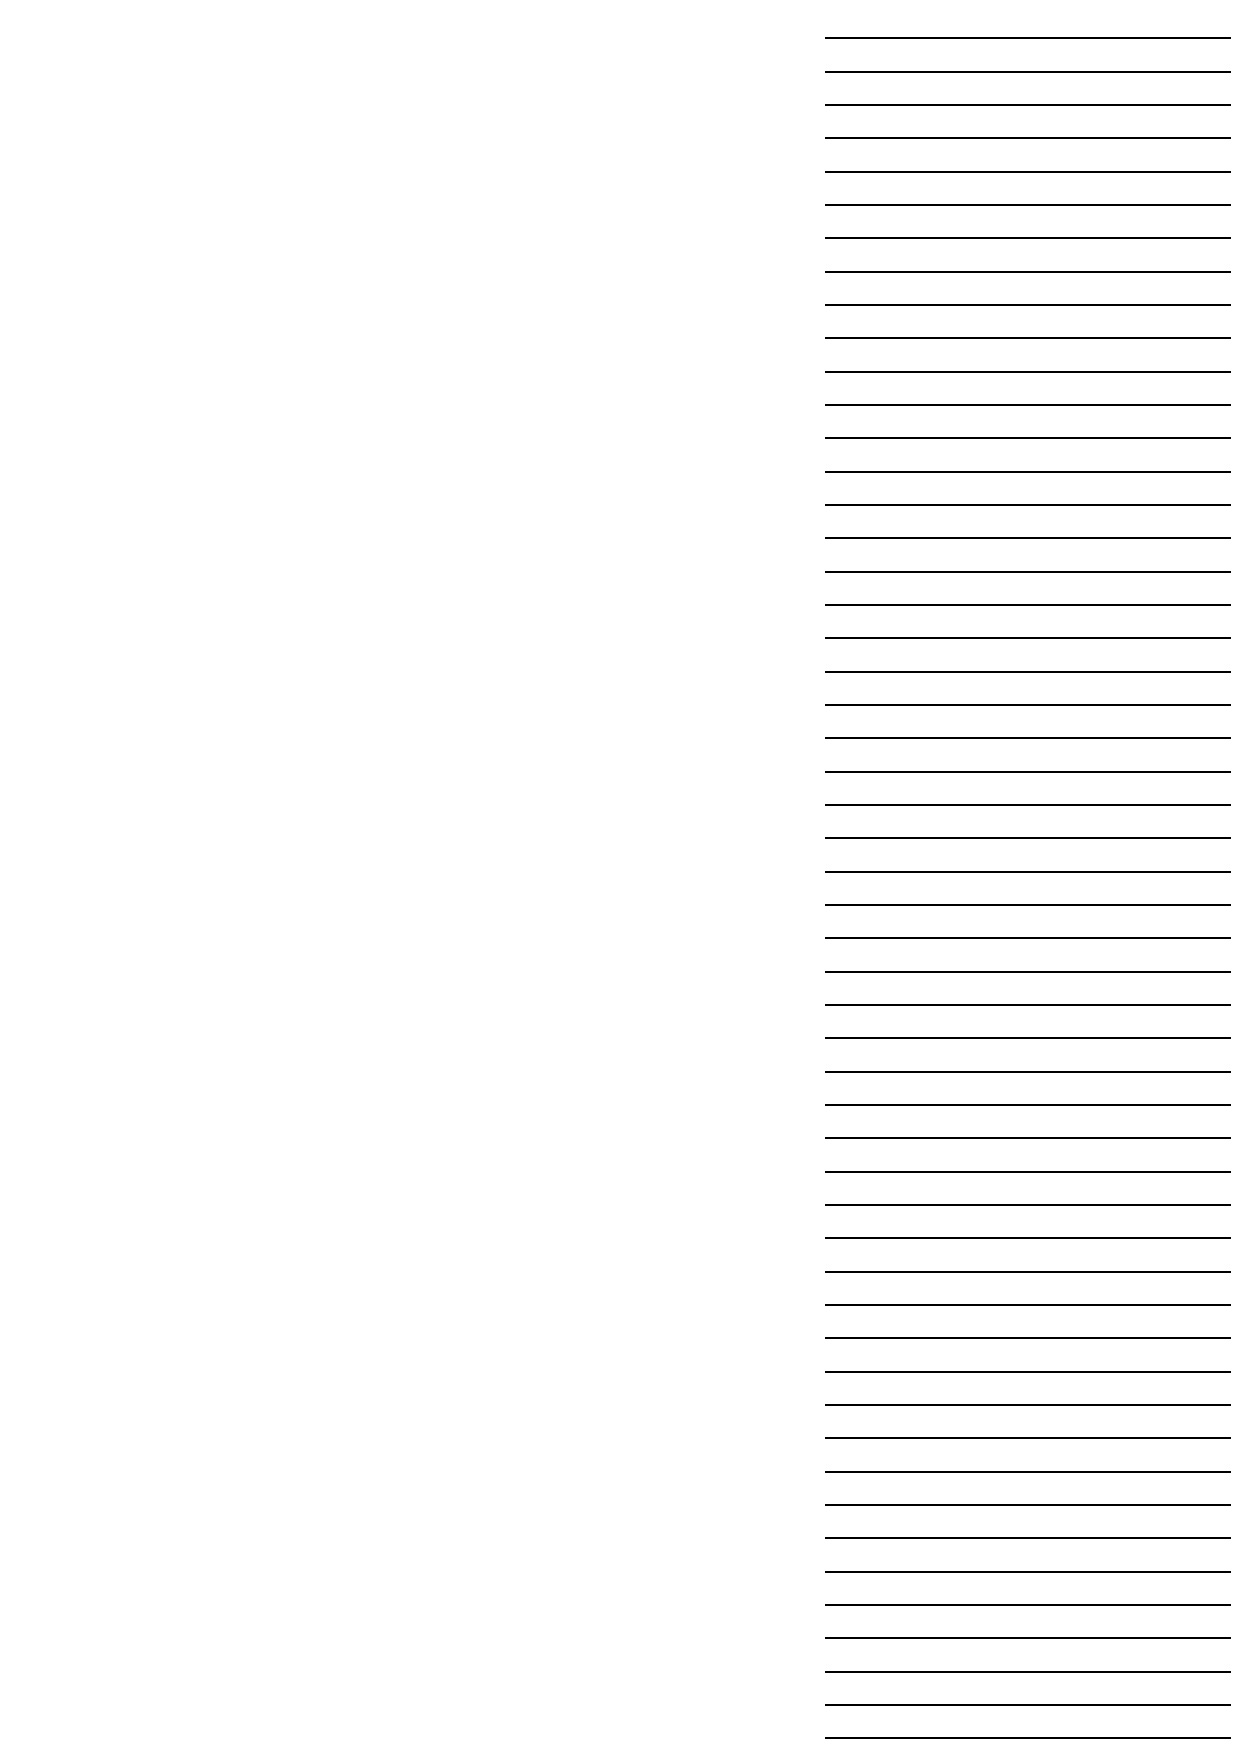
\includegraphics{template_files/backgroundlines}}}


\usepackage{tikz}
\usepackage{pgfplots}
\usepackage{tikzscale}
\usepackage{graphicx}
\usepackage{float}
\usepackage{subcaption}
\usepackage{comment}
\usepackage{units}
\usetikzlibrary{external}\tikzexternalize


\title{H2b: Variational Monte Carlo}
\author{Victor Nilsson and Simon Nilsson}
\date{\today}

\begin{document}

\newgeometry{top=2cm,bottom=2cm,left=2cm,right=2cm}

\begin{titlepage}

\setcounter{page}{0}

\begin{center}
{\huge \bf \color{red} NB: The graded, first version of the report must be
                           returned if you hand in a second time! } \\
\vspace{3cm}
\makeatletter
{ \huge \@title } \\
\vspace{1cm}
{ \Large \@author }\\
\vspace{1cm}
{ \Large \@date }\\
\makeatother
\end{center}

\vfill

\begin{flushright}
{\Large
\begin{tabular}{|c|c|c|}
\hline
Task N\textsuperscript{\underline{o}} & Points & Avail.\ points \\ \hline
\hspace{3cm} & \hspace{3cm} & \hspace{3cm} \\ \hline
~ & ~ & ~ \\ \hline
~ & ~ & ~ \\ \hline
~ & ~ & ~ \\ \hline
~ & ~ & ~ \\ \hline
~ & ~ & ~ \\ \hline
~ & ~ & ~ \\ \hline
~ & ~ & ~ \\ \hline
$\sum$ & ~ & ~ \\
\hline
\end{tabular}}
\end{flushright}

\end{titlepage}

\newgeometry{top=2cm,bottom=2cm,left=1.5cm,right=7.4cm}


\section*{Introduction}



\section*{Problem 1}

\begin{figure}[H]
    \centering
    \captionsetup[subfigure]{justification=centering}
    \begin{subfigure}[b]{0.40\textwidth}
        \centering
        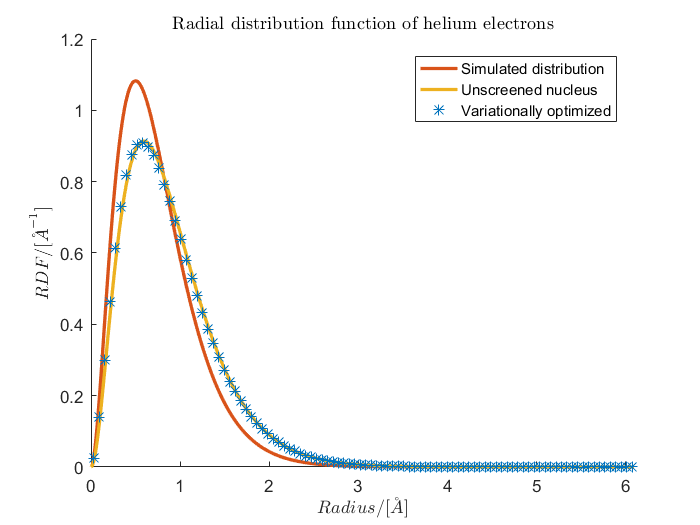
\includegraphics[width=\textwidth]{graphics/task1/radius.png}
    \end{subfigure}
    \begin{subfigure}[b]{0.40\textwidth}
        \centering
        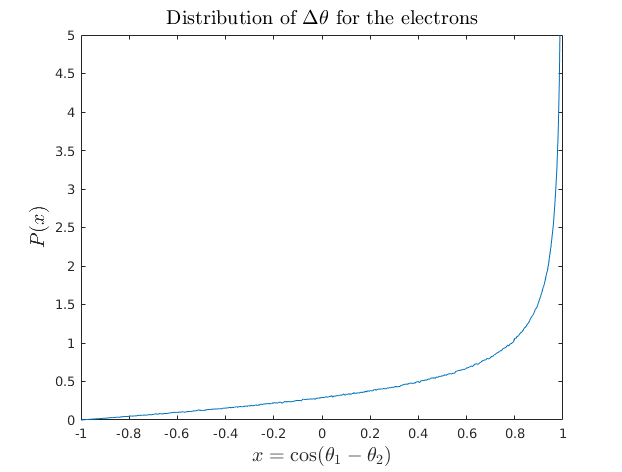
\includegraphics[width=\textwidth]{graphics/task1/angle_diff_dist.png}
    \end{subfigure}
    \caption{\textit{Left:} Simulated and calculated radial distribution function for the two electrons in the helium atom. \textit{Right:} The distribution of cosine of the relative $\theta$ angle for the two electrons.}
    \label{fig:RDF}
\end{figure}

As we can see in (Fig.~\ref{fig:RDF}) we can see that out radial distribution looks like the variationally optimized distribution.

\section*{Problem 2}

\begin{figure}[H]
	\centering
	\captionsetup[subfigure]{justification=centering}
	\begin{subfigure}[b]{0.4\textwidth}
		\centering
		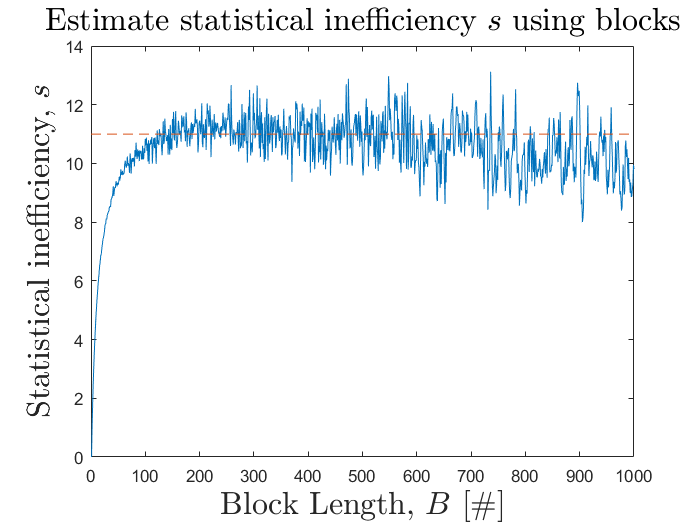
\includegraphics[width=\textwidth]{graphics/task2/block_error.png}
	\end{subfigure}
	\caption{Estimation of the statistical inefficiency based on different block lengths}
	\label{fig:block_error}
\end{figure}


\section*{Problem 3}


\begin{figure}[H]
	\centering
	\captionsetup[subfigure]{justification=centering}
	\begin{subfigure}[b]{0.4\textwidth}
		\centering
		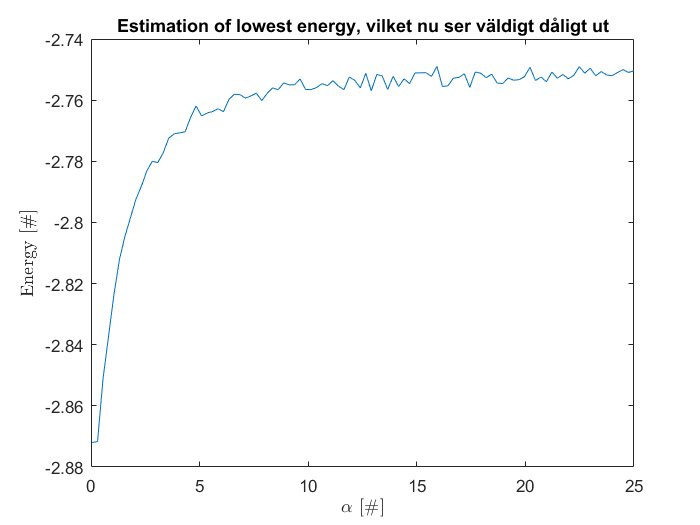
\includegraphics[width=\textwidth]{graphics/task3/lowest_energy.png}
	\end{subfigure}
	\caption{Estimation of the statistical inefficiency based on different block lengths}
	\label{fig:optimize_alpha}
\end{figure}



\section*{Problem 4}

\begin{equation}
	\psi_t(r_1,r_2) = e^{-2r_1}e^{-2r_2}e^{\frac{r_{12}}{2(1+\alpha r_{12})}}
\end{equation}

\begin{equation}
	\nabla \alpha \ln{\psi_t(r_1,r_2)} = -\frac{r_{12}^2}{2(1+\alpha r_{12})^2}
\end{equation}

$\beta = 0.75$
$\alpha_{min}=0.142553129000000$
$E_{min}=-2.891044220000000$

\section*{Problem 5}

$E_min=-2.878146$


\appendix
\section{Source code}

\subsection{\texttt{Task1/main.c}}
%\lstinputlisting[language=c, numbers=left]{../code/Task1/main.c}

\end{document}
